\newpage
\subsection{Chosen Drone}
\begin{wrapfigure}{r}{0.3\textwidth}
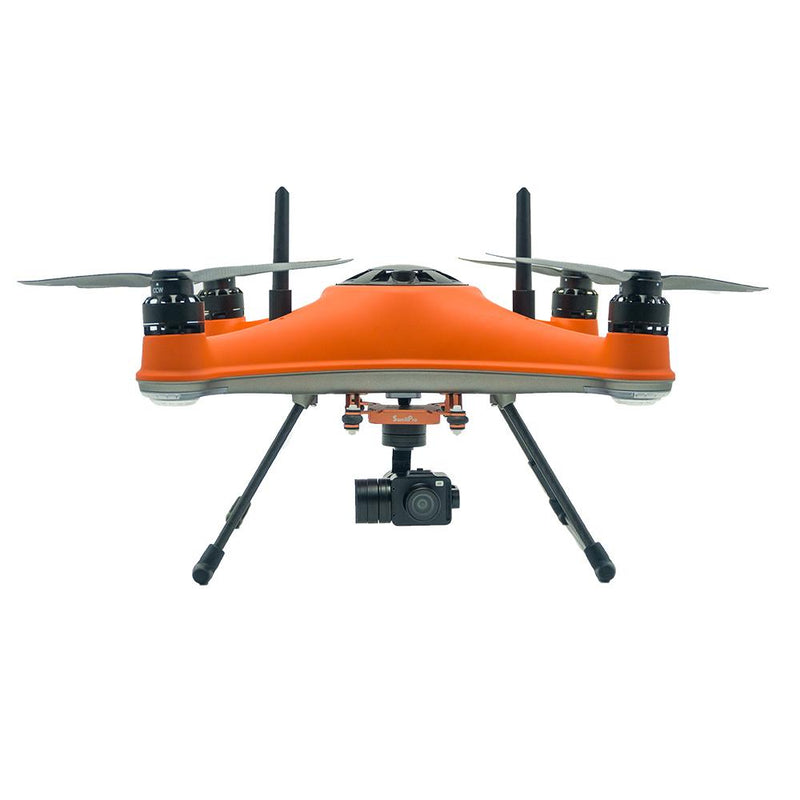
\includegraphics[width=1\linewidth]{070_design/chosendrone/21_splashdrone4.png}
\caption{SplashDrone 4 \cite{splashdrone4}}
\end{wrapfigure}
As seen in the Preliminary Research Report in Appendix A, \cite{prr} it turns out that the SwellPro SplashDrone 4 is the best option as a base for the project. While a \gls{DIY} drone was considered, building a custom drone solution that was also waterproof seemed out of this project's scope.\\

As mentioned, the drone can land in the water, which opens up the possibilities of \gls{2D}/\gls{3D} water quality measurements. The drone has ports on the bottom for connecting hardware via a serial connection. 

This makes it possible to power a microcontroller (using a step down converter), sensors, and even a servo winch. The latter can help when building a sensor enclosure which can move to any depth of water, creating \gls{3D} water quality measurements.

\begin{figure}[h]
\centering
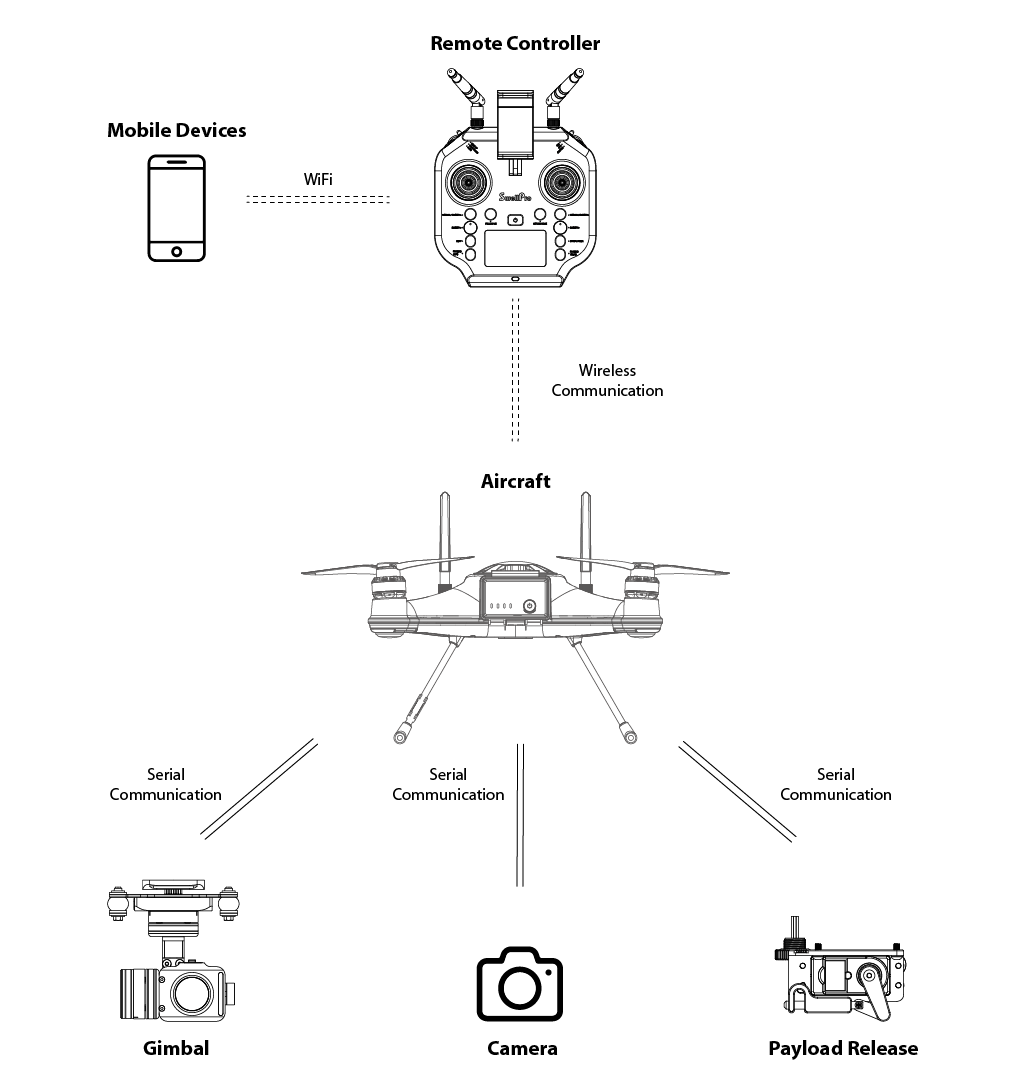
\includegraphics[scale=1.1]{070_design/chosendrone/22_controldiagram.png}
\caption{Flight Control Communication Protocol Diagram \cite{swellpronotion}}
\end{figure}

The drone and its add-ons are entirely controllable via a \gls{TCP} and serial connection one can have with its remote controller. Data is received and transmitted via Swellpro's "Flight Control Communication Protocol". \cite{swellpronotion}